% t-SNE Lecture - Slides 1-9 (Revised Slide 8 for aesthetics)
\documentclass{beamer}
\usetheme{Madrid}
\usecolortheme{seahorse}
\usepackage{amsmath}
\usepackage{amssymb}
\usepackage{graphicx}
\usepackage{tikz}
\usetikzlibrary{shapes.geometric, arrows.meta, positioning}

% Define custom colors for consistency
\definecolor{upcblue}{RGB}{0,123,199}
\definecolor{upcgray}{RGB}{100,100,100}
\definecolor{highlight}{RGB}{255,127,0}

% Adjust beamer margins to prevent truncation
\setbeamersize{text margin left=5mm,text margin right=5mm}

\begin{document}

% SLIDE 1: Title Slide
\begin{frame}[plain]
\vspace{0.5cm}
\begin{center}
{\LARGE \textcolor{upcblue}{\textbf{Nonlinear Dimensionality Reduction:}}}\\[0.2cm]
{\huge \textcolor{upcblue}{\textbf{t-Stochastic Neighbor Embedding}}}\\[0.2cm]
{\huge \textcolor{upcblue}{\textbf{(t-SNE)}}}\\[1cm]

{\large \textbf{Prof. Endri Raco}}\\[0.2cm]
{\normalsize Polytechnic University of Tirana}\\[0.1cm]
{\small \textit{Erasmus+ Exchange Professor}}\\[0.8cm]

{\large \textcolor{upcgray}{Advanced Multivariate Analysis}}\\[0.2cm]
{\normalsize Polytechnic University of Catalonia (UPC)}\\[0.3cm]
{\normalsize October 15, 2025}
\end{center}

\vspace{0.3cm}
\begin{center}
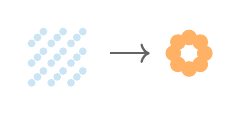
\begin{tikzpicture}[scale=0.25]
% 3D point cloud on the left
\foreach \x in {0,1,2}
    \foreach \y in {0,1,2}
        \foreach \z in {0,1,2}
            \node[circle, fill=upcblue!20, inner sep=1pt] at (\x+\z*0.3,\y+\z*0.3) {};
            
% Arrow indicating transformation
\draw[->, thick, upcgray] (4,1.5) -- (6,1.5);

% 2D circular arrangement on the right
\foreach \angle in {0,45,...,315}
    \node[circle, fill=highlight!60, inner sep=2pt] at ({8+0.8*cos(\angle)},{1.5+0.8*sin(\angle)}) {};
\end{tikzpicture}
\end{center}
\end{frame}

% SLIDE 2: Welcome and Overview
\begin{frame}{Welcome to Advanced Multivariate Analysis}
\vspace{-0.2cm}
{\color{upcblue}\textbf{Today's Journey}}\\[0.2cm]
\begin{itemize}
    \setlength\itemsep{0.3em}
    \item \textbf{2-hour deep dive} into t-SNE
    \item \textbf{Mathematical foundations} to practical insights
    \item \textbf{Three key parts:}
    \begin{enumerate}
        \item SNE - The original idea
        \item t-SNE - Solving the crowding problem  
        \item Hyperparameters \& interpretation
    \end{enumerate}
\end{itemize}

\vspace{0.3cm}
\begin{center}
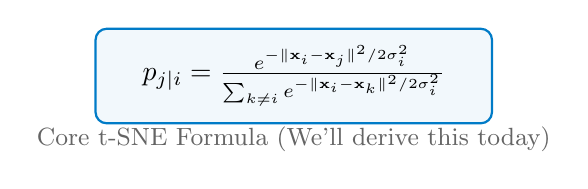
\begin{tikzpicture}[scale=0.8]
    \node[draw=upcblue, thick, rounded corners, 
          minimum width=5cm, minimum height=1.2cm,
          fill=upcblue!5] at (0,0) {
        \begin{minipage}{4.8cm}
        \centering
        $p_{j|i} = \frac{e^{-\|\mathbf{x}_i - \mathbf{x}_j\|^2/2\sigma_i^2}}{\sum_{k \neq i} e^{-\|\mathbf{x}_i - \mathbf{x}_k\|^2/2\sigma_i^2}}$
        \end{minipage}
    };
    \node at (0,-1) {\small \textcolor{upcgray}{Core t-SNE Formula (We'll derive this today)}};
\end{tikzpicture}
\end{center}
\end{frame}

% SLIDE 3: The Challenge of High-Dimensional Data
\begin{frame}{The Curse of Dimensionality}
\vspace{-0.3cm}
\begin{columns}[T]
\begin{column}{0.48\textwidth}
\textbf{\color{upcblue}Our Intuition Works Here:}

\begin{center}
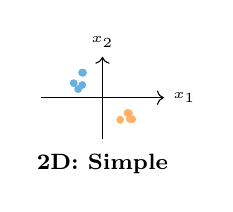
\begin{tikzpicture}[scale=0.65]
    % 2D scatter plot
    \node at (0,-1.3) {\footnotesize \textbf{2D: Simple}};
    \draw[->] (-1.2,0) -- (1.2,0) node[right] {\tiny $x_1$};
    \draw[->] (0,-0.8) -- (0,0.8) node[above] {\tiny $x_2$};
    
    % Cluster 1
    \foreach \i in {1,...,5} {
        \node[circle, fill=upcblue!60, inner sep=1pt] at ({-0.5+0.2*rand},{0.3+0.2*rand}) {};
    }
    % Cluster 2
    \foreach \i in {1,...,5} {
        \node[circle, fill=highlight!60, inner sep=1pt] at ({0.5+0.2*rand},{-0.3+0.2*rand}) {};
    }
\end{tikzpicture}
\end{center}

\begin{center}
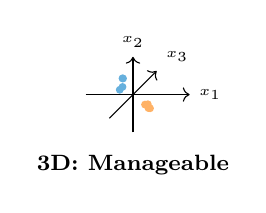
\begin{tikzpicture}[scale=0.6]
    % 3D scatter plot
    \node at (0,-1.5) {\footnotesize \textbf{3D: Manageable}};
    \draw[->] (-1,0) -- (1.2,0) node[right] {\tiny $x_1$};
    \draw[->] (0,-0.8) -- (0,0.8) node[above] {\tiny $x_2$};
    \draw[->] (-0.5,-0.5) -- (0.5,0.5) node[above right] {\tiny $x_3$};
    
    % 3D clusters
    \foreach \i in {1,...,4} {
        \node[circle, fill=upcblue!60, inner sep=1pt] at ({-0.3+0.15*rand},{0.2+0.15*rand}) {};
    }
    \foreach \i in {1,...,4} {
        \node[circle, fill=highlight!60, inner sep=1pt] at ({0.3+0.15*rand},{-0.2+0.15*rand}) {};
    }
\end{tikzpicture}
\end{center}
\end{column}

\begin{column}{0.48\textwidth}
\textbf{\color{upcblue}But Not Here:}

\begin{center}
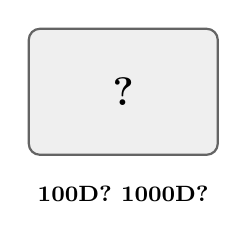
\begin{tikzpicture}
    \draw[upcgray, thick, rounded corners, fill=upcgray!10] 
          (-1.2,-0.8) rectangle (1.2,0.8);
    \node at (0,0) {\Large \textbf{?}};
    \node at (0,-1.3) {\footnotesize \textbf{100D? 1000D?}};
\end{tikzpicture}
\end{center}

\vspace{0.3cm}
\textcolor{upcgray}{\textbf{Problems:}}
\begin{itemize}
    \small
    \item \textcolor{highlight}{Distance concentration}
    \item \textcolor{highlight}{Volume:} $V_n(r) \propto r^n$
    \item \textcolor{highlight}{Sparse data}
\end{itemize}

\vspace{0.2cm}
\centering
\small\textit{\color{upcblue}``Geometric intuition fails''}
\end{column}
\end{columns}
\end{frame}

% SLIDE 4: Why Reduce Dimensions?
\begin{frame}{Goals of Dimensionality Reduction}
\vspace{-0.3cm}
\begin{columns}[T]
\begin{column}{0.48\textwidth}
\textbf{\color{upcblue}Goal 1: Visualization}

\begin{center}
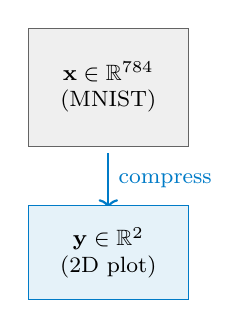
\begin{tikzpicture}[scale=0.7]
    % High-dimensional
    \node[draw=upcgray, minimum width=2cm, minimum height=1.5cm, fill=upcgray!10] 
          at (0,0) {
        \begin{minipage}{1.8cm}
        \centering
        \footnotesize
        $\mathbf{x} \in \mathbb{R}^{784}$\\
        (MNIST)
        \end{minipage}
    };
    
    % Arrow
    \draw[->, thick, upcblue] (0,-1.2) -- (0,-2.2) 
          node[midway, right] {\footnotesize compress};
    
    % Low-dimensional
    \node[draw=upcblue, minimum width=2cm, minimum height=1.2cm, fill=upcblue!10] 
          at (0,-3) {
        \begin{minipage}{1.8cm}
        \centering
        \footnotesize
        $\mathbf{y} \in \mathbb{R}^{2}$\\
        (2D plot)
        \end{minipage}
    };
\end{tikzpicture}
\end{center}

\small
\textcolor{upcgray}{\textbf{Key:}} ``See'' hidden structure
\end{column}

\begin{column}{0.48\textwidth}
\textbf{\color{upcblue}Goal 2: Feature Extraction}

\begin{center}
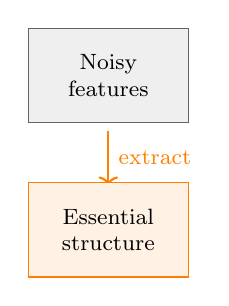
\begin{tikzpicture}[scale=0.7]
    % Original
    \node[draw=upcgray, minimum width=2cm, minimum height=1.2cm, fill=upcgray!10] 
          at (0,0) {
        \begin{minipage}{1.8cm}
        \centering
        \footnotesize
        Noisy\\features
        \end{minipage}
    };
    
    % Arrow
    \draw[->, thick, highlight] (0,-1) -- (0,-2) 
          node[midway, right] {\footnotesize extract};
    
    % Essential
    \node[draw=highlight, minimum width=2cm, minimum height=1.2cm, fill=highlight!10] 
          at (0,-2.8) {
        \begin{minipage}{1.8cm}
        \centering
        \footnotesize
        Essential\\structure
        \end{minipage}
    };
\end{tikzpicture}
\end{center}

\small
\textcolor{upcgray}{\textbf{Benefits:}}
\begin{itemize}
    \footnotesize
    \item Noise reduction
    \item Efficiency
    \item Better ML
\end{itemize}
\end{column}
\end{columns}

\vspace{0.3cm}
\begin{center}
\colorbox{upcblue!10}{
\begin{minipage}{0.85\textwidth}
\centering
\small\textbf{Challenge:} Preserve relationships while reducing dimensions
\end{minipage}
}
\end{center}
\end{frame}

% SLIDE 5: The Limits of Linear Projections
\begin{frame}{When Linear Methods Falter}
\vspace{-0.3cm}
\begin{columns}[T]
\begin{column}{0.48\textwidth}
\textbf{\color{upcblue}Swiss Roll Dataset}

\begin{center}
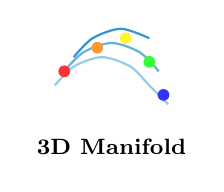
\begin{tikzpicture}[scale=0.6]
    % Swiss Roll curves
    \draw[thick, upcblue!40] plot[smooth, tension=0.5] 
          coordinates {(-1.2,0) (-0.8,0.4) (-0.2,0.6) (0.4,0.4) (0.8,0) (1.2,-0.4)};
    \draw[thick, upcblue!60] plot[smooth, tension=0.5] 
          coordinates {(-1,0.3) (-0.6,0.7) (0,0.9) (0.6,0.7) (1,0.3)};
    \draw[thick, upcblue!80] plot[smooth, tension=0.5] 
          coordinates {(-0.8,0.6) (-0.4,1) (0.2,1.2) (0.8,1)};
    
    % Points with colors
    \node[circle, fill=red!80, inner sep=1.5pt] at (-1,0.3) {};
    \node[circle, fill=orange!80, inner sep=1.5pt] at (-0.3,0.8) {};
    \node[circle, fill=yellow!80, inner sep=1.5pt] at (0.3,1) {};
    \node[circle, fill=green!80, inner sep=1.5pt] at (0.8,0.5) {};
    \node[circle, fill=blue!80, inner sep=1.5pt] at (1.1,-0.2) {};
    
    \node at (0,-1.3) {\footnotesize \textbf{3D Manifold}};
\end{tikzpicture}
\end{center}

\small
\textcolor{upcgray}{\textbf{True Structure:}}\\
\footnotesize 2D manifold in 3D space
\end{column}

\begin{column}{0.48\textwidth}
\textbf{\color{upcblue}PCA Projection}

\begin{center}
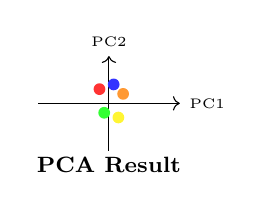
\begin{tikzpicture}[scale=0.6]
    % PCA axes
    \draw[->] (-1.5,0) -- (1.5,0) node[right] {\tiny PC1};
    \draw[->] (0,-1) -- (0,1) node[above] {\tiny PC2};
    
    % Mixed colors - PCA failure
    \node[circle, fill=red!80, inner sep=1.5pt] at (-0.2,0.3) {};
    \node[circle, fill=blue!80, inner sep=1.5pt] at (0.1,0.4) {};
    \node[circle, fill=orange!80, inner sep=1.5pt] at (0.3,0.2) {};
    \node[circle, fill=green!80, inner sep=1.5pt] at (-0.1,-0.2) {};
    \node[circle, fill=yellow!80, inner sep=1.5pt] at (0.2,-0.3) {};
    
    \node at (0,-1.3) {\footnotesize \textbf{PCA Result}};
\end{tikzpicture}
\end{center}

\small
\textcolor{highlight}{\textbf{Problem:}}\\
\footnotesize Preserves variance,\\
\footnotesize destroys local structure
\end{column}
\end{columns}

\vspace{0.2cm}
\begin{center}
\colorbox{highlight!20}{
\begin{minipage}{0.85\textwidth}
\centering
\small\textit{Need methods that preserve \textbf{local relationships}}
\end{minipage}
}
\end{center}
\end{frame}

% SLIDE 6: The Manifold Hypothesis
\begin{frame}{The Manifold Hypothesis}
\vspace{-0.3cm}
\begin{center}
\colorbox{upcblue!10}{
\begin{minipage}{0.9\textwidth}
\centering
\textit{``High-dimensional data often lies on or near}\\
\textit{a much lower-dimensional manifold''}
\end{minipage}
}
\end{center}

\vspace{0.3cm}
\begin{columns}[T]
\begin{column}{0.48\textwidth}
\textbf{\color{upcblue}Example: Earth's Surface}

\begin{center}
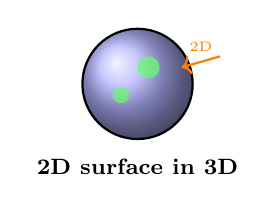
\begin{tikzpicture}[scale=0.7]
    % Earth sphere
    \shade[ball color=blue!30] (0,0) circle (1cm);
    \draw[thick] (0,0) circle (1cm);
    
    % Continents
    \fill[green!60, opacity=0.7] (0.2,0.3) circle (0.2cm);
    \fill[green!60, opacity=0.7] (-0.3,-0.2) circle (0.15cm);
    
    % Arrow
    \draw[->, thick, highlight] (1.5,0.5) -- (0.8,0.3) 
          node[above, midway] {\tiny 2D};
    
    \node at (0,-1.5) {\footnotesize \textbf{2D surface in 3D}};
\end{tikzpicture}
\end{center}
\end{column}

\begin{column}{0.48\textwidth}
\textbf{\color{upcblue}Mathematical Form}

\small
Data: $\mathbf{X} = \{\mathbf{x}_1, ..., \mathbf{x}_n\}$\\
where $\mathbf{x}_i \in \mathbb{R}^D$

\vspace{0.2cm}
\textbf{Assumption:}\\
$\exists$ manifold $\mathcal{M}$ with dim $d \ll D$:

$$\mathbf{x}_i \approx f(\mathbf{z}_i) + \epsilon_i$$

\footnotesize
\begin{itemize}
    \item $\mathbf{z}_i \in \mathbb{R}^d$ (low-dim)
    \item $f: \mathbb{R}^d \rightarrow \mathbb{R}^D$
    \item $\epsilon_i$ (noise)
\end{itemize}
\end{column}
\end{columns}

\vspace{0.2cm}
\begin{center}
\colorbox{upcgray!10}{
\begin{minipage}{0.85\textwidth}
\centering
\small\textbf{Goal:} Uncover this hidden low-dimensional structure
\end{minipage}
}
\end{center}
\end{frame}

% SLIDE 7: A Glimpse of t-SNE
\begin{frame}{Preserving Neighborhoods: t-SNE in Action}
\vspace{-0.2cm}
\begin{columns}[T]
\begin{column}{0.48\textwidth}
\textbf{\color{upcblue}PCA on MNIST Digits}

\begin{center}
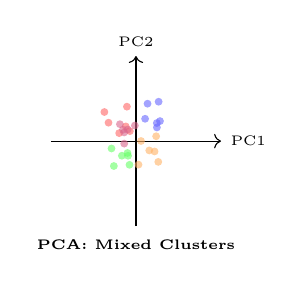
\begin{tikzpicture}[scale=0.6]
    % PCA axes
    \draw[->] (-1.8,0) -- (1.8,0) node[right] {\tiny PC1};
    \draw[->] (0,-1.8) -- (0,1.8) node[above] {\tiny PC2};
    
    % Overlapping clusters - PCA
    \foreach \x/\y/\c in {-0.4/0.4/red!60, 0.3/0.5/blue!60, -0.2/-0.3/green!60, 
                          0.3/-0.2/orange!60, -0.3/0.1/purple!60} {
        \foreach \i in {1,...,6} {
            \pgfmathsetmacro{\rx}{0.35*rand}
            \pgfmathsetmacro{\ry}{0.35*rand}
            \node[circle, fill=\c, inner sep=1pt, opacity=0.6] at (\x+\rx,\y+\ry) {};
        }
    }
    
    \node at (0,-2.2) {\tiny \textbf{PCA: Mixed Clusters}};
\end{tikzpicture}
\end{center}

\footnotesize
\textcolor{upcgray}{\textbf{Problems:}}
\begin{itemize}
    \tiny
    \item Classes overlap significantly
    \item Linear projection limitations
    \item Poor cluster separation
\end{itemize}
\end{column}

\begin{column}{0.48\textwidth}
\textbf{\color{upcblue}t-SNE on MNIST Digits}

\begin{center}
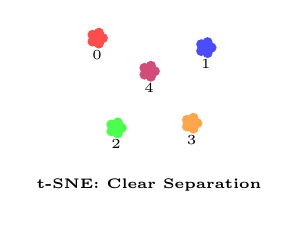
\begin{tikzpicture}[scale=0.6]
    % t-SNE well-separated clusters
    \foreach \x/\y/\c/\l in {-1.1/0.9/red!70/0, 1.2/0.7/blue!70/1, 
                              -0.7/-1/green!70/2, 0.9/-0.9/orange!70/3, 
                              0/0.2/purple!70/4} {
        % Tight cluster
        \foreach \i in {1,...,5} {
            \pgfmathsetmacro{\angle}{360*\i/5}
            \node[circle, fill=\c, inner sep=1.3pt] at ({\x+0.12*cos(\angle)},{\y+0.12*sin(\angle)}) {};
        }
        \node[circle, fill=\c, inner sep=1.3pt] at (\x,\y) {};
        \node at (\x,\y-0.35) {\tiny \l};
    }
    
    \node at (0,-2.2) {\tiny \textbf{t-SNE: Clear Separation}};
\end{tikzpicture}
\end{center}

\footnotesize
\textcolor{highlight}{\textbf{Advantages:}}
\begin{itemize}
    \tiny
    \item Distinct clusters
    \item Preserves local structure
    \item Reveals true relationships
\end{itemize}
\end{column}
\end{columns}

\vspace{0.15cm}
\begin{center}
\colorbox{upcblue!10}{
\begin{minipage}{0.8\textwidth}
\centering
\footnotesize\textit{``t-SNE focuses on preserving \textbf{local neighborhood structure}''}\\
\footnotesize\textit{Similar points in high-D $\rightarrow$ nearby points in low-D}
\end{minipage}
}
\end{center}
\end{frame}

% SLIDE 8: Lecture Outline (Aesthetic Revision)
\begin{frame}{Today's Journey: From Theory to Mastery}
\vspace{1cm} 
\centering
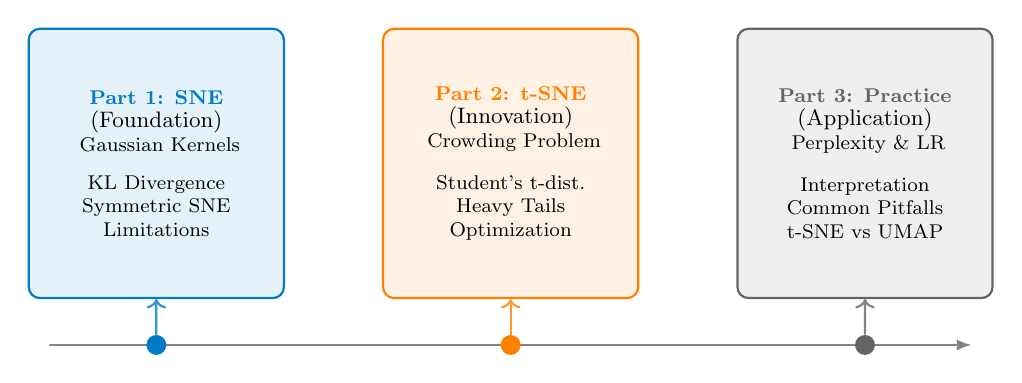
\begin{tikzpicture}[
    scale=0.9, transform shape,
    % Styles
    box/.style={
        draw, thick, rounded corners,
        minimum width=3.6cm, minimum height=3.8cm,
        align=center, font=\footnotesize,
        inner sep=5pt
    },
    point/.style={
        circle, fill, minimum size=8pt, inner sep=0pt
    },
    timeline/.style={
        -latex, thick, upcgray!80, line cap=round
    }
]

% The main timeline arrow
\draw[timeline] (-6.5,0) -- (6.5,0);

% Part 1: SNE
\node[point, fill=upcblue] (p1) at (-5,0) {};
\node[box, draw=upcblue, fill=upcblue!10, above=0.5cm of p1] (b1) {
    \textbf{\color{upcblue}Part 1: SNE} \\
    \small(Foundation) \\ \vspace{2mm}
    Gaussian Kernels \\
    KL Divergence \\
    Symmetric SNE \\
    Limitations
};
\draw[->, thick, upcblue!80] (p1.north) -- (b1.south);

% Part 2: t-SNE
\node[point, fill=highlight] (p2) at (0,0) {};
\node[box, draw=highlight, fill=highlight!10, above=0.5cm of p2] (b2) {
    \textbf{\color{highlight}Part 2: t-SNE} \\
    \small(Innovation) \\ \vspace{2mm}
    Crowding Problem \\
    Student's t-dist. \\
    Heavy Tails \\
    Optimization
};
\draw[->, thick, highlight!80] (p2.north) -- (b2.south);

% Part 3: Practice
\node[point, fill=upcgray] (p3) at (5,0) {};
\node[box, draw=upcgray, fill=upcgray!10, above=0.5cm of p3] (b3) {
    \textbf{\color{upcgray}Part 3: Practice} \\
    \small(Application) \\ \vspace{2mm}
    Perplexity \& LR \\
    Interpretation \\
    Common Pitfalls \\
    t-SNE vs UMAP
};
\draw[->, thick, upcgray!80] (p3.north) -- (b3.south);

\end{tikzpicture}
\end{frame}


% SLIDE 9: Let's Begin - The Core Idea
\begin{frame}{From Distances to Probabilities: The Core Idea}
\vspace{-0.2cm}

\begin{center}
\colorbox{upcblue!10}{
\begin{minipage}{0.85\textwidth}
\centering
\textbf{Central Insight:} Convert distances between points into probabilities\\
that represent neighborhood relationships
\end{minipage}
}
\end{center}

\vspace{0.3cm}
\begin{columns}[T]
\begin{column}{0.48\textwidth}
\textbf{\color{upcblue}Traditional Approach}
\vspace{0.2cm}

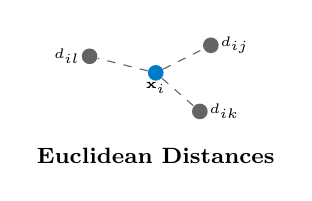
\begin{tikzpicture}[scale=0.7]
    % Distance-based
    \node[circle, fill=upcblue, inner sep=2pt] (c) at (0,0) {};
    \node[below] at (c) {\tiny $\mathbf{x}_i$};
    
    \node[circle, fill=upcgray, inner sep=2pt] (p1) at (1,0.5) {};
    \node[right] at (p1) {\tiny $d_{ij}$};
    
    \node[circle, fill=upcgray, inner sep=2pt] (p2) at (0.8,-0.7) {};
    \node[right] at (p2) {\tiny $d_{ik}$};
    
    \node[circle, fill=upcgray, inner sep=2pt] (p3) at (-1.2,0.3) {};
    \node[left] at (p3) {\tiny $d_{il}$};
    
    \draw[dashed, upcgray] (c) -- (p1);
    \draw[dashed, upcgray] (c) -- (p2);
    \draw[dashed, upcgray] (c) -- (p3);
    
    \node at (0,-1.5) {\footnotesize \textbf{Euclidean Distances}};
\end{tikzpicture}

\footnotesize
Problem: How to weight different distances?
\end{column}

\begin{column}{0.48\textwidth}
\textbf{\color{upcblue}SNE/t-SNE Approach}
\vspace{0.2cm}

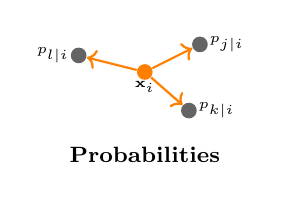
\begin{tikzpicture}[scale=0.7]
    % Probability-based
    \node[circle, fill=highlight, inner sep=2pt] (c) at (0,0) {};
    \node[below] at (c) {\tiny $\mathbf{x}_i$};
    
    \node[circle, fill=upcgray, inner sep=2pt] (p1) at (1,0.5) {};
    \node[right] at (p1) {\tiny $p_{j|i}$};
    
    \node[circle, fill=upcgray, inner sep=2pt] (p2) at (0.8,-0.7) {};
    \node[right] at (p2) {\tiny $p_{k|i}$};
    
    \node[circle, fill=upcgray, inner sep=2pt] (p3) at (-1.2,0.3) {};
    \node[left] at (p3) {\tiny $p_{l|i}$};
    
    \draw[->, highlight, thick] (c) -- (p1);
    \draw[->, highlight, thick] (c) -- (p2);
    \draw[->, highlight, thick] (c) -- (p3);
    
    \node at (0,-1.5) {\footnotesize \textbf{Probabilities}};
\end{tikzpicture}

\footnotesize
Solution: Probabilities naturally normalize!
\end{column}
\end{columns}

\vspace{0.3cm}
\begin{center}
\colorbox{highlight!20}{
\begin{minipage}{0.85\textwidth}
\centering
\footnotesize\textit{``What is the probability that point $i$ would pick point $j$ as its neighbor?''}
\end{minipage}
}
\end{center}
\end{frame}

\end{document}